\chapter{Abstraction, Act 1}


\section*{Where we're going}

The examples of modeling that we've discussed in the previous chapter and in studio -- 
feline high-rise syndrome, box manufacturing -- 
focused on understanding the very big picture of modeling:  what we mean when we talk about ``abstraction'', a ``model'', ``implementation'',  ``prediction'', ``validation'', and ``doing work'' with a model.  

\begin{marginfigure}
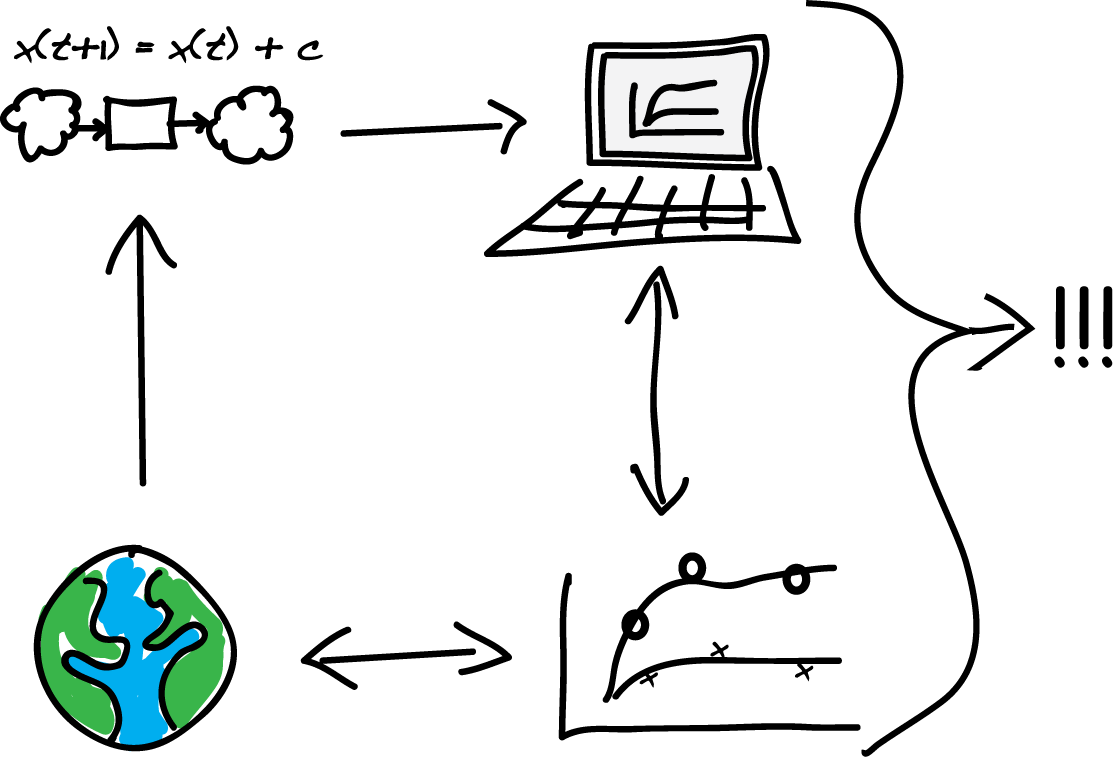
\includegraphics[width=6cm]{figs/ModsimDiagram}
\caption{The Modeling Process.  Can you identify ``abstraction'', a ``model'', ``implementation'',  ``prediction'', ``validation'', and ``doing work'' ? 
 }
\end{marginfigure}
In the case of feline high-rise syndrome we made a distinction between the simplest kind of model of all -- the implicit mental model -- and more formal, but still highly qualitative models of behavior for a physical system.  These models allowed us to make simple predictions (which, in many cases, were not consistent with observed behavior); iterating on these models in light of this validation failure allowed us to generate a qualitative model that explains the physical behavior we observe when Fluffy falls out of a tree and lives to tell the tale.  

The box manufacturing model was more quantitative -- we came up with an actual mathematical representation of the model, as opposed to a cartoon-based representation -- but like the feline high-rise syndrome case, it required abstraction, analysis, validation , and also involved doing design work as opposed to explanatory or predictive work.  And, like the cat example, the model we came up with could certainly be made more accurate, if we thought that was important for the work we wished to do.  Note, of course, that ``more accurate'' does not necessarily mean ``better'' -- ``better'' only makes sense in the context of asking what kind of work you want to do with the model, and whether the model is an appropriate one for that application.

In this chapter, we will begin looking at a broad class of models that deal with systems that evolve in time.  Indeed, this entire class focuses primarily on modeling such {\it dynamic} systems.   We'll begin by introducing formalisms that will allow us to implement our models both analytically and in simulation.  To introduce these formalisms, we'll be confining ourselves in this chapter to one broad kind of system as well -- populations that evolve in time -- but the ideas we'll deal with apply to many other systems as well.

This chapter deals only with the process of {\it abstracting} from a physical system to a model (or a set of models); in subsequent chapters we'll see how to implement these abstractions in code, how to implement them analytically, and ultimately how to validate and do work with them.  

\section{Example Physical System: Elephants in Southern Africa}

As noted above, this chapter focuses on the formalisms associated with abstracting from a physical system to a model.  In order to situate that formalism, let's start out by identifying a physical system we might be interested in modeling.  I've always liked elephants, and it turns out that there are many people who are interested in understanding the populations of elephants:

\begin{marginfigure}
%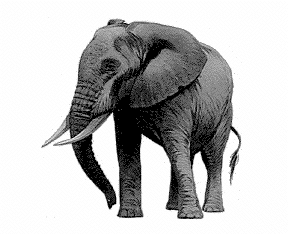
\includegraphics[width=6cm]{figs/elephant}
\caption{An elephant.  From {\tt cksinfo.com}}
\end{marginfigure}

\begin{quote}
During the last century, the number of African elephant (Loxodonta africana) 
declined dramatically as a result of over-hunting, poaching for ivory and, 
more recently, the loss of habitat area due to encroachment of the human population. 
In some areas, however, the trend to declining numbers was reversed after the elephant was 
placed on Appendix 1 of the Convention for International Trade in Endangered Species 
(CITES) and a worldwide ban was imposed on the sale of ivory. Unfortunately, the resulting 
recovery in elephant numbers within both National and privately owned game parks poses 
a threat to the survival of many other species. Indeed, when elephant numbers exceed the 
carrying capacity of a game park, the gradual destruction of vegetation and habitat is 
catastrophic and, if left unchecked, is only arrested when the elephants themselves
 begin to die of starvation. Over the last 30 years, it became generally accepted that 
 the best way to prevent this boom-and-bust scenario and, in addition keep epidemic 
 diseases under control, was to maintain elephant numbers below the carrying capacity 
 by culling. During the 1990s, however, popular opinion turned against culling as a 
 means of controlling elephant populations and the focus shifted instead to translocating 
 animals from areas of high to areas of low population density. Self-evidently, while 
 relocation may be a useful way to control elephant numbers in relatively small 
 parks, it is unrealistic to expect to relocate thousands of animals per year to keep the 
 population under control in the large parks, for example, in northern Botswana. \\
 \flushright{Ben Colenbrander {\tt  http://elephantpopulationcontrol.library.uu.nl/ }}
\end{quote}
 
Given what Mr. Colenbrander has to say, it seems clear that there might be good reason to have a model of elephant populations -- after all, it's a lot easier to deal with virtual elephants than real elephants in exploring different policy options!  So, what do you say we build a model of elephant populations?

For the sake of argument, let's assume we are interested in modeling elephant population in a game park, in order to (1) ensure the continued survival of the elephants (important for the elephants, and also for the profitability of the park), and (2) in order to make sure that the number of elephants does not get too high.  


\section{Formalism \#1: Stock and flow diagrams}

\subsection{An Example}

Now, in modeling, it is ALWAYS a good idea to start with the simplest model that we can possibly imagine.  Then, once you think you have a simple model that makes sense, add complexity in small pinches until the model is {\it just} complicated enough to do the work you want the model to do.

\begin{marginfigure}
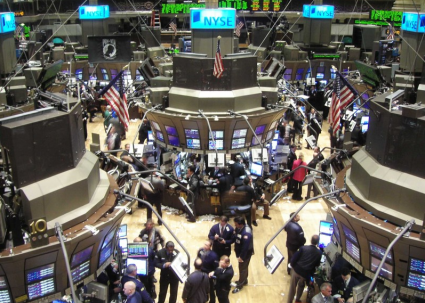
\includegraphics[width=6cm]{figs/stockmarket}
\caption{No, not that kind of stock. From {\tt http://www.dvmcfnllc.com}}
\end{marginfigure}

So we're going to start REALLY simple.  We'll assume that elephants enter the park by being born, and they leave the park by dying.  

We're also going to assume that the system we are modeling consists of live elephants inside the physical boundary of the park:  we are not keeping track of elephants outside of the park, nor are we keeping track of dead elephants or elephant fetuses.

An aside here:  We just made a really important statement:  we defined our {\it system}.  We drew a dotted line around ``live elephants in the game park'', and divided the universe into the system and the surroundings:  the elephants in the park are the system; the food supply, the hunters; and the elephants outside the park are all part of the surroundings.  In modeling, we will make assumptions about the surroundings in order to make predictions about what happens to the system.    

To represent our simple model, we're going to introduce a piece of formalism called a {\it stock and flow diagram} that can be pretty helpful for expressing your models -- particularly as the models get more complex.  Let's start by looking at the diagram, and then we'll deconstruct it a bit.

Here's the diagram.

%\begin{figure}[h!]
\beforefig
\centerline{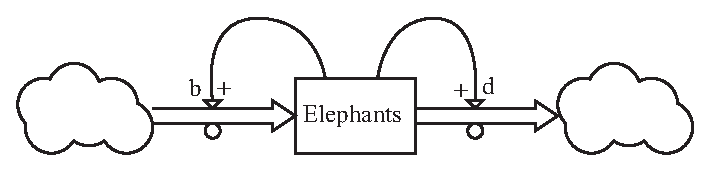
\includegraphics[height=1in]{figs/ElephantStockAndFlow1}}
%\caption{Simple stock and flow diagram, showing elephant populations changing due to birth and death} 
%end{figure}
\afterfig

The diagram basically says the same thing we said before:

\begin{itemize}
\item There are a certain number of elephants in the park.
\item Over time, the number of elephants can change due to two processes: birth and death.
\item The number of elephants born each year is proportional to the number of elephants currently alive.
\item The number of elephants that die each year is also proportional to the number of elephants currently alive.
\end{itemize}

Stock and flow diagrams contain a number of key elements, including (not surprisingly) {\it stocks}, {\it flows}, {\it information}, and {\it sources and sinks}.  Each of these elements is discussed briefly below.


\subsection{Stocks}

In stock and flow diagrams, stocks are represented with a box, like this:

%\begin{figure}[h!]
\beforefig
\centerline{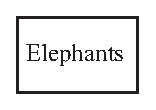
\includegraphics[height=.5in]{figs/Stock}}
%\caption{Representation of a stock. } %end{figure}
\afterfig

Stocks represent the physical stuff that we are keeping track of in an accounting sense -- i.e., we are watching how much of the stuff there is over time. A stock is the kind of stuff that you can measure an amount of, or that is in some sense countable.  This is consistent with our common usage of the word stock:  for example, we talk about number of heads of livestock, or the number of barrels of available oil stocks, or the amount of toothpaste that a drugstore has in stock.  Along the same lines, stocks tend to be nouns:  ``elephants'' (how many elephants there are in the game park), ``ice'' (how much ice there is in a freezer), ``stored energy'' (how much energy is stored in a compressed spring).  

In physics, quantities that are {\it extensive} and {\it conserved} \footnote{Extensive quantities are quantities that depend on the number of particles in a the system -- for example, two liters of gas at STP contains more energy and more mass than one liter of gas at STP. Conserved quantities are quantities that only change by going somewhere else -- e.g., the amount of energy in a system can only change if energy somehow enters or leaves the system.}  tend to be stocks -- e.g., energy, momentum, charge.  And stocks therefore tend to have units of number, or mass, or volume, or moles, or joules.

It is worth contrasting quantities that are stocks with some quantities that are not stocks.  Frequently it is tempting to call an {\it intensive} quantity, like temperature, a stock -- and if you look around in the literature, you'll find that people do this fairly frequently.  I recommend that youresist this temptation. Intensive quantities are quantities that are properties of the material within the system, but which do not depend on the number of particles in the system.  Temperature and density are good examples -- two liters of gas at STP has the same temperature and density as one liter of gas at STP.  Both of these are properties of the material, but not of the amount of the material -- and it would not make sense to talk about increasing the amount of temperature in the system, nor would it make sense to talk about temperature being conserved.  

This is a subtle point -- you'll want to think about it some more later in the course. It primarily comes into play when you have two stocks in a system that are connected to each other.  For example, if you were keeping track of both elephants in the park and elephants outside the park, it would make sense to have those two stocks connected:

%\begin{figure}[h!]
\beforefig
\centerline{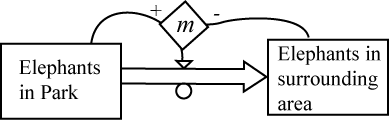
\includegraphics[height=.6in]{figs/TwoStockElephantsExample1}}
%\caption{Example of a two stock model.}
%end{figure}
\afterfig
This indicates that the number of elephants leaving the park due to migration is the same as the number of elephants entering the surrounding area.    This is clearly not the case for intensive quantities like temperature. 


\subsection{Flows}

\begin{marginfigure}
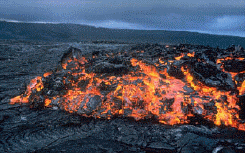
\includegraphics[width=6cm]{figs/lavaflow}
\caption{Nor do we mean this kind of flow. Well, maybe we could, if we were keeping track of lava as a stock...}
\end{marginfigure}
Flows are represented with a double arrow, like this:

%\begin{figure}[h!]
\beforefig
\centerline{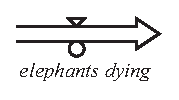
\includegraphics[height=.4in]{figs/Flow}}
%\caption{Symbol representing a flow -- a process by which a stock changes. } %end{figure}
\afterfig


Flows represent the processes by which a stock changes.  Since they represent processes, they often are verbs or phrases:  ``dying'', ``melting''.  The units of flows tend to be in stock per unit time (e.g., number per year, kilograms per second).  And while stocks have memory, flows do not: if you doubled the temperature 
in a room, the amount of ice in the room would not change instantaneously, but the rate of ice melting would.  

The circle/triangle symbol represents a valve -- i.e., the thing that controls the flow.  When there is more than one thing controlling the flow, the flow is the {\em product} of the control quantities.  So, above, the number of elephants that die each year is a product of the number of elephants and $d$, the elephant death rate (i.e., the chance that a given elephant dies each year, or the fraction of the total elephant population that dies each year).  We'll see some more examples of this later.


\subsection{Information}

Now, flows often depend on information, either about the level of stocks inside the system, or about the value of variables that are outside the system.  This informational dependence is represented by a single-lined arrows, like this:

%\begin{figure}[h!]
\beforefig
\centerline{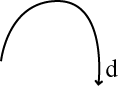
\includegraphics[height=.5in]{figs/Information}} 
%%\caption{ } %end{figure}
\afterfig

which says that the number of elephants dying each year is proportional to what the current elephant population is, and that the proportionality constant is the parameter $d$.

Often information arrows will have a sign associated with them: a $+$ sign indicates that raising the quantity increases the flow; a $-$ sign indicates that increasing the quantity tends to reduce the flow.  

\subsection{Sources and Sinks}
Finally, when we define the boundaries of the system that we are modeling, we also have to account for the world outside of the boundaries using sources and sinks, which are represented with a cloud:

\begin{marginfigure}
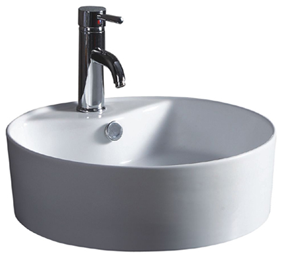
\includegraphics[width=6cm]{figs/bathroomsink}
\caption{The joke sucked the first two times, too.}
\end{marginfigure}

%\begin{figure}[h!]
\beforefig
\centerline{
\includegraphics[height=.5in]{figs/sink}}
%\caption{ } %end{figure}
\afterfig

The idea of a source or a sink is that it has an unlimited capacity to absorb or provide material:  for example, there are an unlimited number of potential elephant babies somewhere in elephant heaven, and there is unlimited space in the elephant graveyard for dead elephants.  We make these unlimited because they are outside of the system boundaries, so we've chosen not to model them.

\subsection{Functional Dependencies, Parameters, and Exogenous Variables}

Now we will take two steps in making the model more complex.  First, Let's add the fact that there is a limited amount of food in the park, so that as the population grows, the death rate due to starvation grows as well.  Second, we'll add an additional death mechanism:  poaching.

%\begin{figure}[h!]
\beforefig
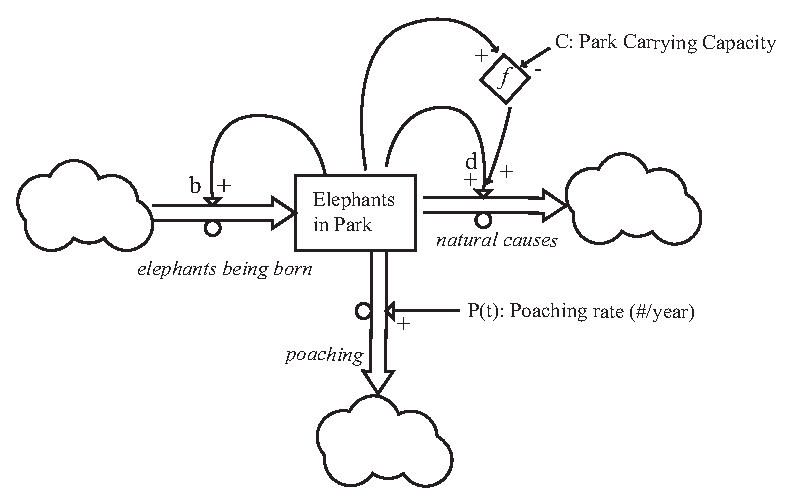
\includegraphics[height=3in]{figs/ElephantStockAndFlow2}
%\caption{ } %end{figure}
\afterfig


We've introduced two new bits of formalism: the diamond, and the plain text variables that originate information flows (e.g., ``P(t): Poaching rate'').  The diamond indicates that there is an additional {\it function} -- something like the available food per elephant --  which controls the death rate.  This function depends on a parameter, the carrying capacity of the park, and also on the number of elephants. Looking at the signs on the arrows, we see that increasing the carrying capacity has the effect of reducing the function, while increasing the number of elephants increases the function:  larger carrying capacity $\rightarrow$ more food $\rightarrow$ less death from starvation; larger population $\rightarrow$ less food per elephant $\rightarrow$ more death from starvation.  

The plain text variables or functions are {\it parameters}, or {\it exogenous variables}.  Exogenous simply means that they are something that is coming from outside -- i.e., something that the model takes as a given, rather than purports to explain.  We might, for example, assume that the poaching rate changes on a yearly basis -- but we are taking that as an assumption, not something that the model predicts.  Similarly, we might decide that the park has a given carrying capacity  -- but we're not modeling how the carrying capacity depends on the number of elephants.  In some ways, you can think about exogenous variables as being like sources for information -- it's information that is coming from outside the system.

What's the difference between exogenous variables and parameters?  Well, often we talk about parameters as being {\it numbers} that don't change in time, whereas exogenous variables can be functions of time.  But this is a bit of a fine distinction, I think.

A quick comment about the multiple information flows in the above diagram:  the diagram says that the number of elephants that die each year due to natural causes is a product of the number of elephants, the death rate $d$, and the function $f$ that depends on both the number of elephants and the carrying capacity $C$.

\vfill

\pagebreak

\section{Summary of Stock and Flow Components}

\begin{center}
\begin{tabular}{ | p{2cm} | p{3cm} | p{3cm} | p{2cm}  | p{3cm}  |}
Name & Description & Examples & Typical Units & Symbol \\
\hline
Stock & a noun; a quantity with ``memory''; an extensive, conserved quantity & elephants, mass, energy & number, mass, volume, Joules & \vspace{0.1in} 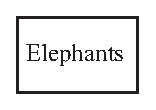
\includegraphics[height=.5in]{figs/Stock} \\

\hline
Flow & a process by which a stock changes, a rate, a verb & dying, evaporating, charging & number per year, grams per second, Joules per hour & \vspace{0.1in} 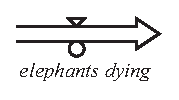
\includegraphics[height=.4in]{figs/Flow}\\

\hline
Information & a quantity, either inside the system or outside the system, that controls a flow & number of elephants, external temperature, voltage level & arbitrary &  \vspace{0.1in}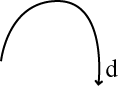
\includegraphics[height=.5in]{figs/Information}\\

\hline
Sinks and Sources & unlimited (and uncounted) stocks that are outside of the system boundary & same as stocks & same as stocks &  \vspace{0.1in}
\includegraphics[height=.5in]{figs/sink} \\

\hline
Functional Dependencies & functions that combine multiple information sources & a birthrate that depends both on carrying capacity and on population & arbitrary &  \vspace{0.1in}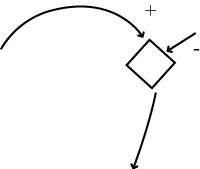
\includegraphics[height=.5in]{figs/functionalDependence} \\

\hline
Exogenous Variables and Parameters& information from outside the system & C, P(t) & arbitrary &  plain text \\

\end{tabular}
\end{center}

\pagebreak

\section{Exercises}

\subsection{Stock or not?}

Which of the following quantities might reasonably be stocks?  Flows?  Neither? Why?

\begin{enumerate}
\item The population of the world
\item The number of educated adults in a country
\item The number of U-238 atoms in a nuclear reactor
\item The pressure level in a nuclear reactor
\item The fraction of battery charge remaining in a laptop battery
\item The power being consumed by a laptop
\item The speed of a runner
\item The kinetic energy of a bullet
\item The number of barrels of oil imported by the U.S. each year
\item The biomass of scallops in the George's Bank fishing area
\item The number of minke whales harvested worldwide each year
\item The reproduction rate of minke whales (number of babies per adult per year)
\item The electric current passing through a wire (i.e., the number of Coulombs of charge passing a given point per unit time)
\item The amount of water in a bathtub
\item The number of liters of water per second flowing out of a faucet
\item The rate of temperature change in a room (degrees C per second)
 \end{enumerate}
 
\subsection{Trees and lawns}

\begin{marginfigure}
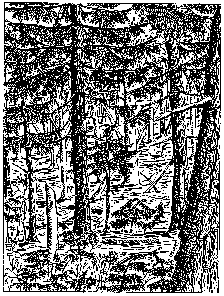
\includegraphics[width=6cm]{figs/forest}
\end{marginfigure}
In the Northeast, the level of forestation has changed wildly over the last two hundred years, due to a variety of processes, both natural and social.   Make a stock and flow diagram that could be used to explain how the number of trees in the Northeast has changed over the last two hundred years.  Keep this pretty simple:  one stock, three or four flows.  Accompany your stock and flow with a bullet list explaining the different flows, information flows, functional dependencies, and exogenous variables.

\section{Formalism \#2: Difference Equations}

\subsection{Discrete-Time vs Continuous-Time}

So far, we've defined the stock and flows for the elephant in the park, but we haven't yet spelled out whether we intend to keep track of elephants in discrete time or in continuous time. If we choose discrete time then we will keep track of the stock in discrete time units (e.g. the elephant population from year to year) and flows tell us about the change in the stock per year (e.g. the number of elephants born each year). In continuous time on the other hand, stocks are defined at all points in time (e.g. we know the elephant population at any moment) and flows tell us about the rate of change of stock (e.g. the rate of change of elephants due to birth). It's up to us to choose either discrete or continuous time, and our choice should depend on the system we are modeling and the work we intend to do. Some stocks like energy seem to be continuously changing in time and thus a discrete model may not be the best choice, while other systems like an elephant population change more slowly and a discrete model may be the best choice.  

For the rest of this module we will use discrete-time models and we now introduce an additional type of model representation appropriate for discrete models: {\it difference equations}. \footnote{Continuous-Time models will be introduced in the next module and will be formalized with differential equations.}

\subsection{Difference equation formalism}

In mathematics, difference equations are a recurrence relation that define a sequence:  the value of every element in the sequence is defined as a function of elements that precede it.  For example, a very simple difference equation is

$$x(t+1) = x(t) + 2$$

If we let $x(0) = 1$, then $x(1) = 3$, $x(2) = 5$, and so on, leading to the sequence $\{ 1, 3, 5, 7, 9, ... \} $.

Note that in order to define the sequence, we must not only define the recurrence relation, we must also define the first value of $x$.

Also note that in the world of mathematics, we tend to start our labeling of a sequence with $t=0$.  Unfortunately (as we'll encounter shortly) in the world of MATLAB, we must start our labeling with an index of $t=1$.   {\it Vive la diff{\' e}rence!} \sidenote{Sorry.  I couldn't resist.  Would you have been able to?}

Although difference equations {\it look} very simple, they in fact can lead to all kinds of crazy behavior.  For example, the difference equation

$$x(t+1) =r x(t)(1-x(t))$$
looks innocent enough, but in fact defines the {\it logistic map}, which yields constant behavior for some values of $r$, periodic behavior for others, and chaotic behavior for still others.
\begin{marginfigure}
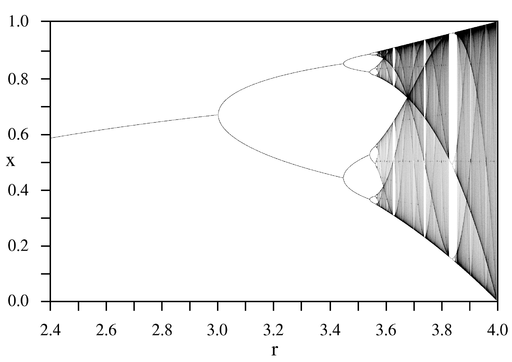
\includegraphics[width=6cm]{figs/bifurcation}
\caption{The bifurcation diagram for the logistic map.  More to come on this!}
\end{marginfigure}


\subsection{Exercise}

Calculate the first 10 terms (i.e., $x(1)$ through $x(10)$) of the logistic map for $r=1$, $r=3.2$, and $r=3.6$.  For all three cases, start with $x(0) = 0.5$.

 

\subsection{Using difference equations for models}

For systems that we wish to model in discrete time, difference equations are an excellent choice mathematically.  Here by ``discrete time'', we mean that we are sampling the system only at particular, discrete instances in time.  For example, if we were modeling the population of birds, we might decide to sample the bird population once a year, and we might decide to build a model that only predicted the bird population at the time of the sampling.  This is not an unreasonable thing to do:  many species breed at a particular time each year, so it makes sense to talk about the number animals born in a particular breeding season.  Similarly, if you wished to model populations of school children, it might make sense to keep track of how many are in first grade, second grade, and so forth, and  so it would make sense to track students by year.  

Returning to our friends the elephants, recall our simple model that looked like this:

%\begin{figure}[h!]
\beforefig
 \centerline{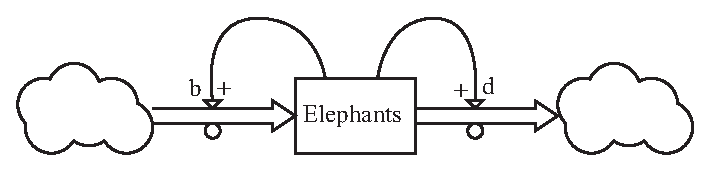
\includegraphics[height=1in]{figs/ElephantStockAndFlow1}}
%\caption{ } %end{figure}
\afterfig

Translating this to a difference equation, we might write

$$E(t+1) = E(t) + b E(t) - d E(t)$$

by which we mean, ``The number of elephants in the game park in year $t+1$ is however many elephants were in the park in year $t$ plus the number born over the course of year $t$, minus the number that died.  The number born  and the number that died in year $t$ are proportional to how many elephants were present in year $t$.''


\subsection{Exercise}

Translate the following stock and flow diagram into a difference equation.  Use a generic function $f(C,E)$ to represent the function of carrying capacity $C$ and elephant population $E$; be sure to define all terms in your difference equation. 

%\begin{figure}[h!]
\beforefig
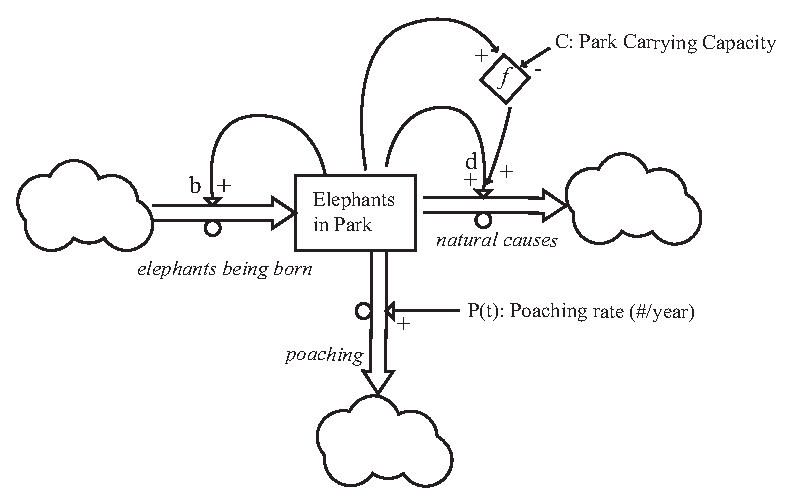
\includegraphics[height=3in]{figs/ElephantStockAndFlow2}
%\caption{ } %end{figure}
\afterfig



\section{Multi-stock models}

Many models involve more than one stock. For example, returning to our friends the elephants, one might want to model both the area surrounding the game park and the actual park:   assuming the fence was low enough for the elephants to jump over, you might get migration between the two areas; at the same time, food supplies and culling policies might be different inside the park than outside, so it could be important to watch both of these stocks separately.

To get started on such a model, you could simply create a stock for the elephants in the surrounding area, and a stock for elephants in the park.  

 \centerline{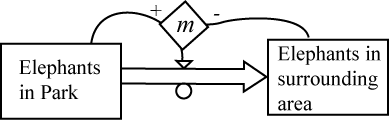
\includegraphics[height=.6in]{figs/TwoStockElephantsExample1}}

Note that in this stock and flow, the flow is shown as migration from the park to the surrounding area.  In principle, that flow could be negative -- in which case more elephants would be moving into the park than moving out -- and it would still be consistent with the stock and flow diagram.  

Since there are two stocks here, we can immediately conclude that we will have two difference equations; since each has one flow, we can also conclude that the difference equations will each have one term to represent the change in the populations.

The difference equations here might look like this:

\begin{eqnarray*}
E(t+1) &=& E(t) -m(E(t),O(t)) \\
O(t+1) &=& O(t) +m(E(t),O(t))
\end{eqnarray*}

where $m$ is a funtion that describes the number of elephants migrating, $E(t)$ is the number of elephants in the park in year $t$, and $O(t)$ is the number of elephants in the region surrounding the park in year $t$.  Note that the flow out of ``Elephants in Park'' is the same as the flow into ``Elephants in surrounding area'' both in the diagram and in the difference equation.

\section{Concluding Remarks}

In this chapter we've introduced two formalisms for abstraction: stock and flow diagrams and difference equations.  

In modeling, stock and flow formalism is extremely helpful as a thinking tool and a communication tool.  It allows you to express fairly complicated ideas without too much overhead, and in a way that captures the ideas in the model visually.  

For example, if you felt that it was important to take into account the carrying capacity, as well as culling within the park, and migration between the park and the surrounding area (and vice-versa), you might draw something like this:

 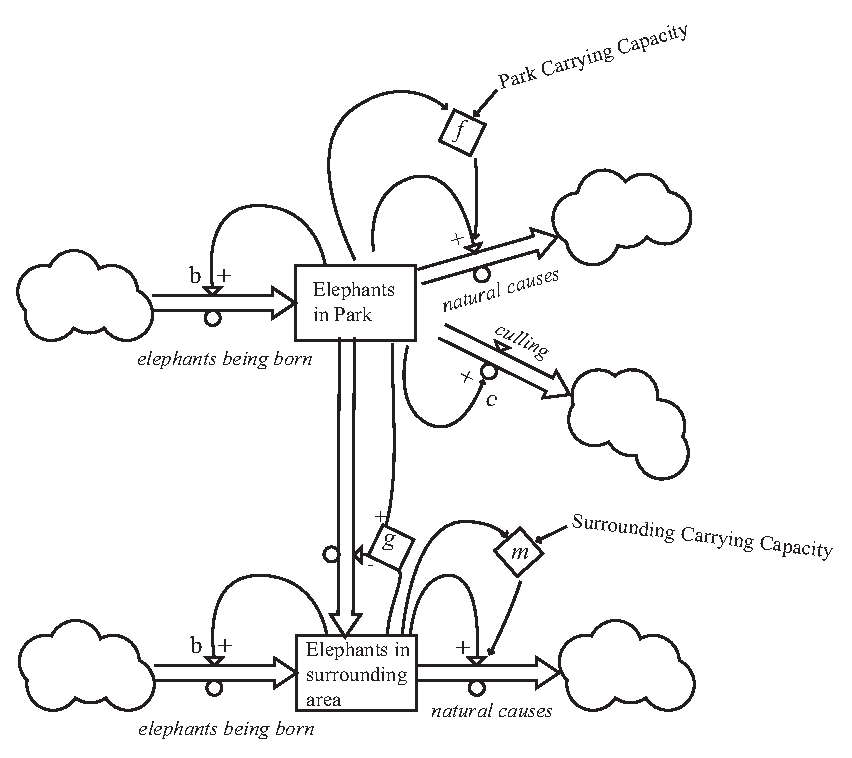
\includegraphics[height=4in]{figs/ElephantStockAndFlow3}

This diagram succinctly expresses, in a graphical way, a large number of effects.  You can see what the ideas in the model are, and what the key relationships are.

On the other hand, stock and flow diagrams don't do much for you in a quantitative sense.  The difference equation formalism allows us to translate stock and flow diagrams into a more formal mathematical model that can be analyzed and/or simulated (as we'll discuss in the upcoming chapters).  

\clearpage

\section{Exercises}

\subsection{Population in the U.K.}
\begin{marginfigure}
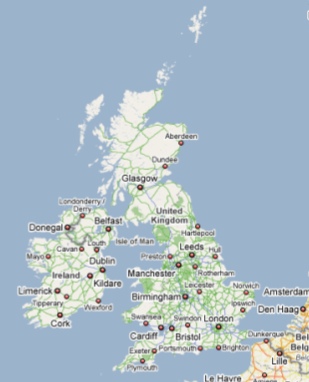
\includegraphics[width=4cm]{figs/ukmap}
\caption{A map of the United Kingdom.}
\end{marginfigure}

 The United Kingdom is a small, but rather proud collection of countries located close to the mainland of Europe. The U.K. consists of England, Scotland, Wales, and Northern Ireland. The U.K. parliament is seated in London, although a devolved parliament in Scotland and devolved assemblies in Wales and Northern Ireland were recently established.\footnote{Strangely enough, England is governed by the U.K. parliament which means that members from Scotland, Wales, and Northern Ireland can vote on issues that only affect England.}



In 2008 the total population of the U.K. was roughly 60 million - about 50 million were in England, about 5 million were in Scotland, about 3 million were in Wales, and about 2 million in Northern Ireland. In the same year, the U.K. instituted a new migration policy - while the people of the U.K. are free to move from country to country as they like, no one is allowed to leave the U.K. or enter the U.K.\footnote{This is what is often known as a {\em word problem} and has absolutely no bearing on reality.} In addition, due to the invention of the deep-fried snickers bar the birth and death rates are now equal and are predicted to remain so for many years to come. Demographers estimate that every year approximately 10\% of the Scottish population will migrate to England. In England, approximately 1\% of residents will move to Scotland every year. In Wales roughly 1000 people will move to England every year. Demographers predict that no one leaves or enters Northern Ireland. 
\begin{enumerate}
\item Draw a stock and flow diagram to model the various UK populations as described above.

\item Write difference equations to model the populations.

\item What is the long-term outlook for Scotland?  For England?
\end{enumerate}

\clearpage

\subsection{Owls}

\begin{marginfigure}
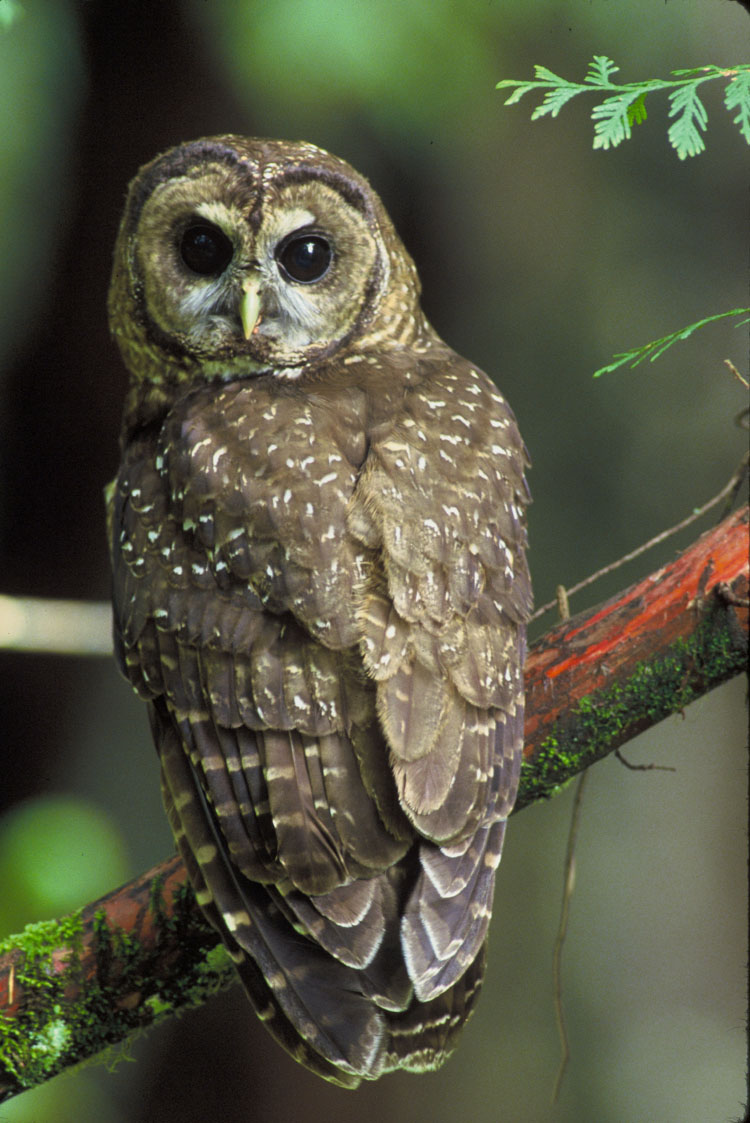
\includegraphics[width=4cm]{figs/owl}
\caption{A spotted owl.  Cute, no?}
\end{marginfigure}
The life cycle of the Northern Spotted Owl divides naturally into three stages: juvenile (up to 1 year), subadult (1 to 2 years), and adult (over 2 years). The owl mates for life during the subadult and adult stages, but only begins to breed as an adult. Using field data from demographic studies, Lamberson et al.\footnote{{\bf A Dynamic Analysis of Northern Spotted Owl Viability in a Fragmented Forest Landscape}, Lamberson, McKelvey, Noon, and Voss, {\em Conservation Biology} 6, 505-512 (1992).} determined that the yearly birth rate was $33\%$, that $18\%$ of the juveniles survive to become adults, that $71\%$ of the subadults survive to become adults and that $94 \%$ of the adults survive every year. 


\begin{enumerate}
\item Draw a stock and flow diagram to model the Northern Spotted Owl population.

\item Write difference equations to model the situation.

\item What is the long-term outlook for the owls? Why?

\item Lamberson's work also indicates that the availability of appropriate nesting trees plays a significant role in determining the birth rate.  Create a new model (stock and flow diagram + difference equations) that takes this effect into account,  and make qualitative predictions about how this will play out.
\end{enumerate}


\clearpage


